%!Mode:: "TeX:UTF-8"
%\begin{frame}
%    \frametitle{OUTLINE}
%    \begin{itemize}    
%        \item
%    \end{itemize}
%\end{frame}

\begin{frame}
    \begin{center}
        \LARGE \tt{GIT}
    \end{center}
\end{frame}

\begin{frame}
    \frametitle{Git基础}
    \begin{itemize}    
        \item 版本控制的概念
            \begin{description}
                \item[版本控制\footnote{\url{http://zh.wikipedia.org/wiki/\%E7\%89\%88\%E6\%9C\%AC\%E6\%8E\%A7\%E5\%88\%B6}}] 
                    是维护工程蓝图的标准作法,
                    能追踪工程蓝图从诞生一直到定案的过程。
                    此外,版本控制也是一种软件工程技巧,
                    借此能在软件开发的过程中,
                    确保由不同人所编辑的同一程式档案都得到同步。
            \end{description}
        \item 关于GIT
            \begin{description}
                \item[Git\footnote{\url{http://zh.wikipedia.org/wiki/Git}}] 
                    是一个由Linus Torvalds
                    为了更好地管理linux内核开发
                    而创立的分布式版本控制/软件配置管理软件。
            \end{description}
        \item 一个重要概念\footnote{\url{http://git-scm.com/book/en/Getting-Started-Git-Basics}}
            \begin{itemize}
                \item Git关心文件数据的整体是否发生变化。
                \item 其他版本管理系统则关心具体内容的差异。
            \end{itemize}
    \end{itemize}
\end{frame}

\begin{frame}
    \frametitle{git的版本控制模型}
    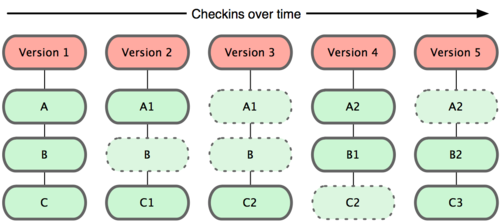
\includegraphics[width=10cm,keepaspectratio]{data/GitRevisionModel.png}

    每个版本都是对这个项目的快照(snapshot)。
\end{frame}

\begin{frame}
    \frametitle{其他系统的版本控制模型}
    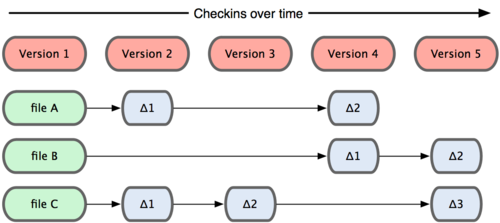
\includegraphics[width=10cm,keepaspectratio]{data/OtherRevisionModel.png}
\end{frame}

\begin{frame}
    \frametitle{分布式工作流程\footnote{\url{http://git-scm.com/book/en/Distributed-Git-Distributed-Workflows}}}
    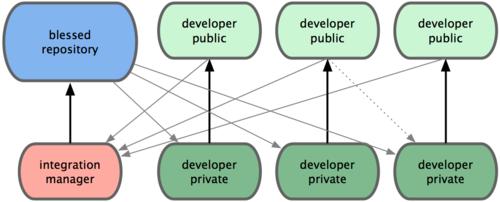
\includegraphics[width=10cm,keepaspectratio]{data/GitDistributedWorkflow.png}
    \begin{block}{我们的开发模式}
        \begin{itemize}
            \item 公共的仓库,由管理员负责
            \item 个人的仓库,由开发者自己管理
            \item 如果要将个人的代码合并如公共的仓库,
                  提交Pull Request,告诉管理员仓库的url和分支名。
        \end{itemize}
    \end{block}
\end{frame}

\begin{frame}
    \frametitle{Git的数据流}
    \begin{columns}
        \column{6.0cm}
            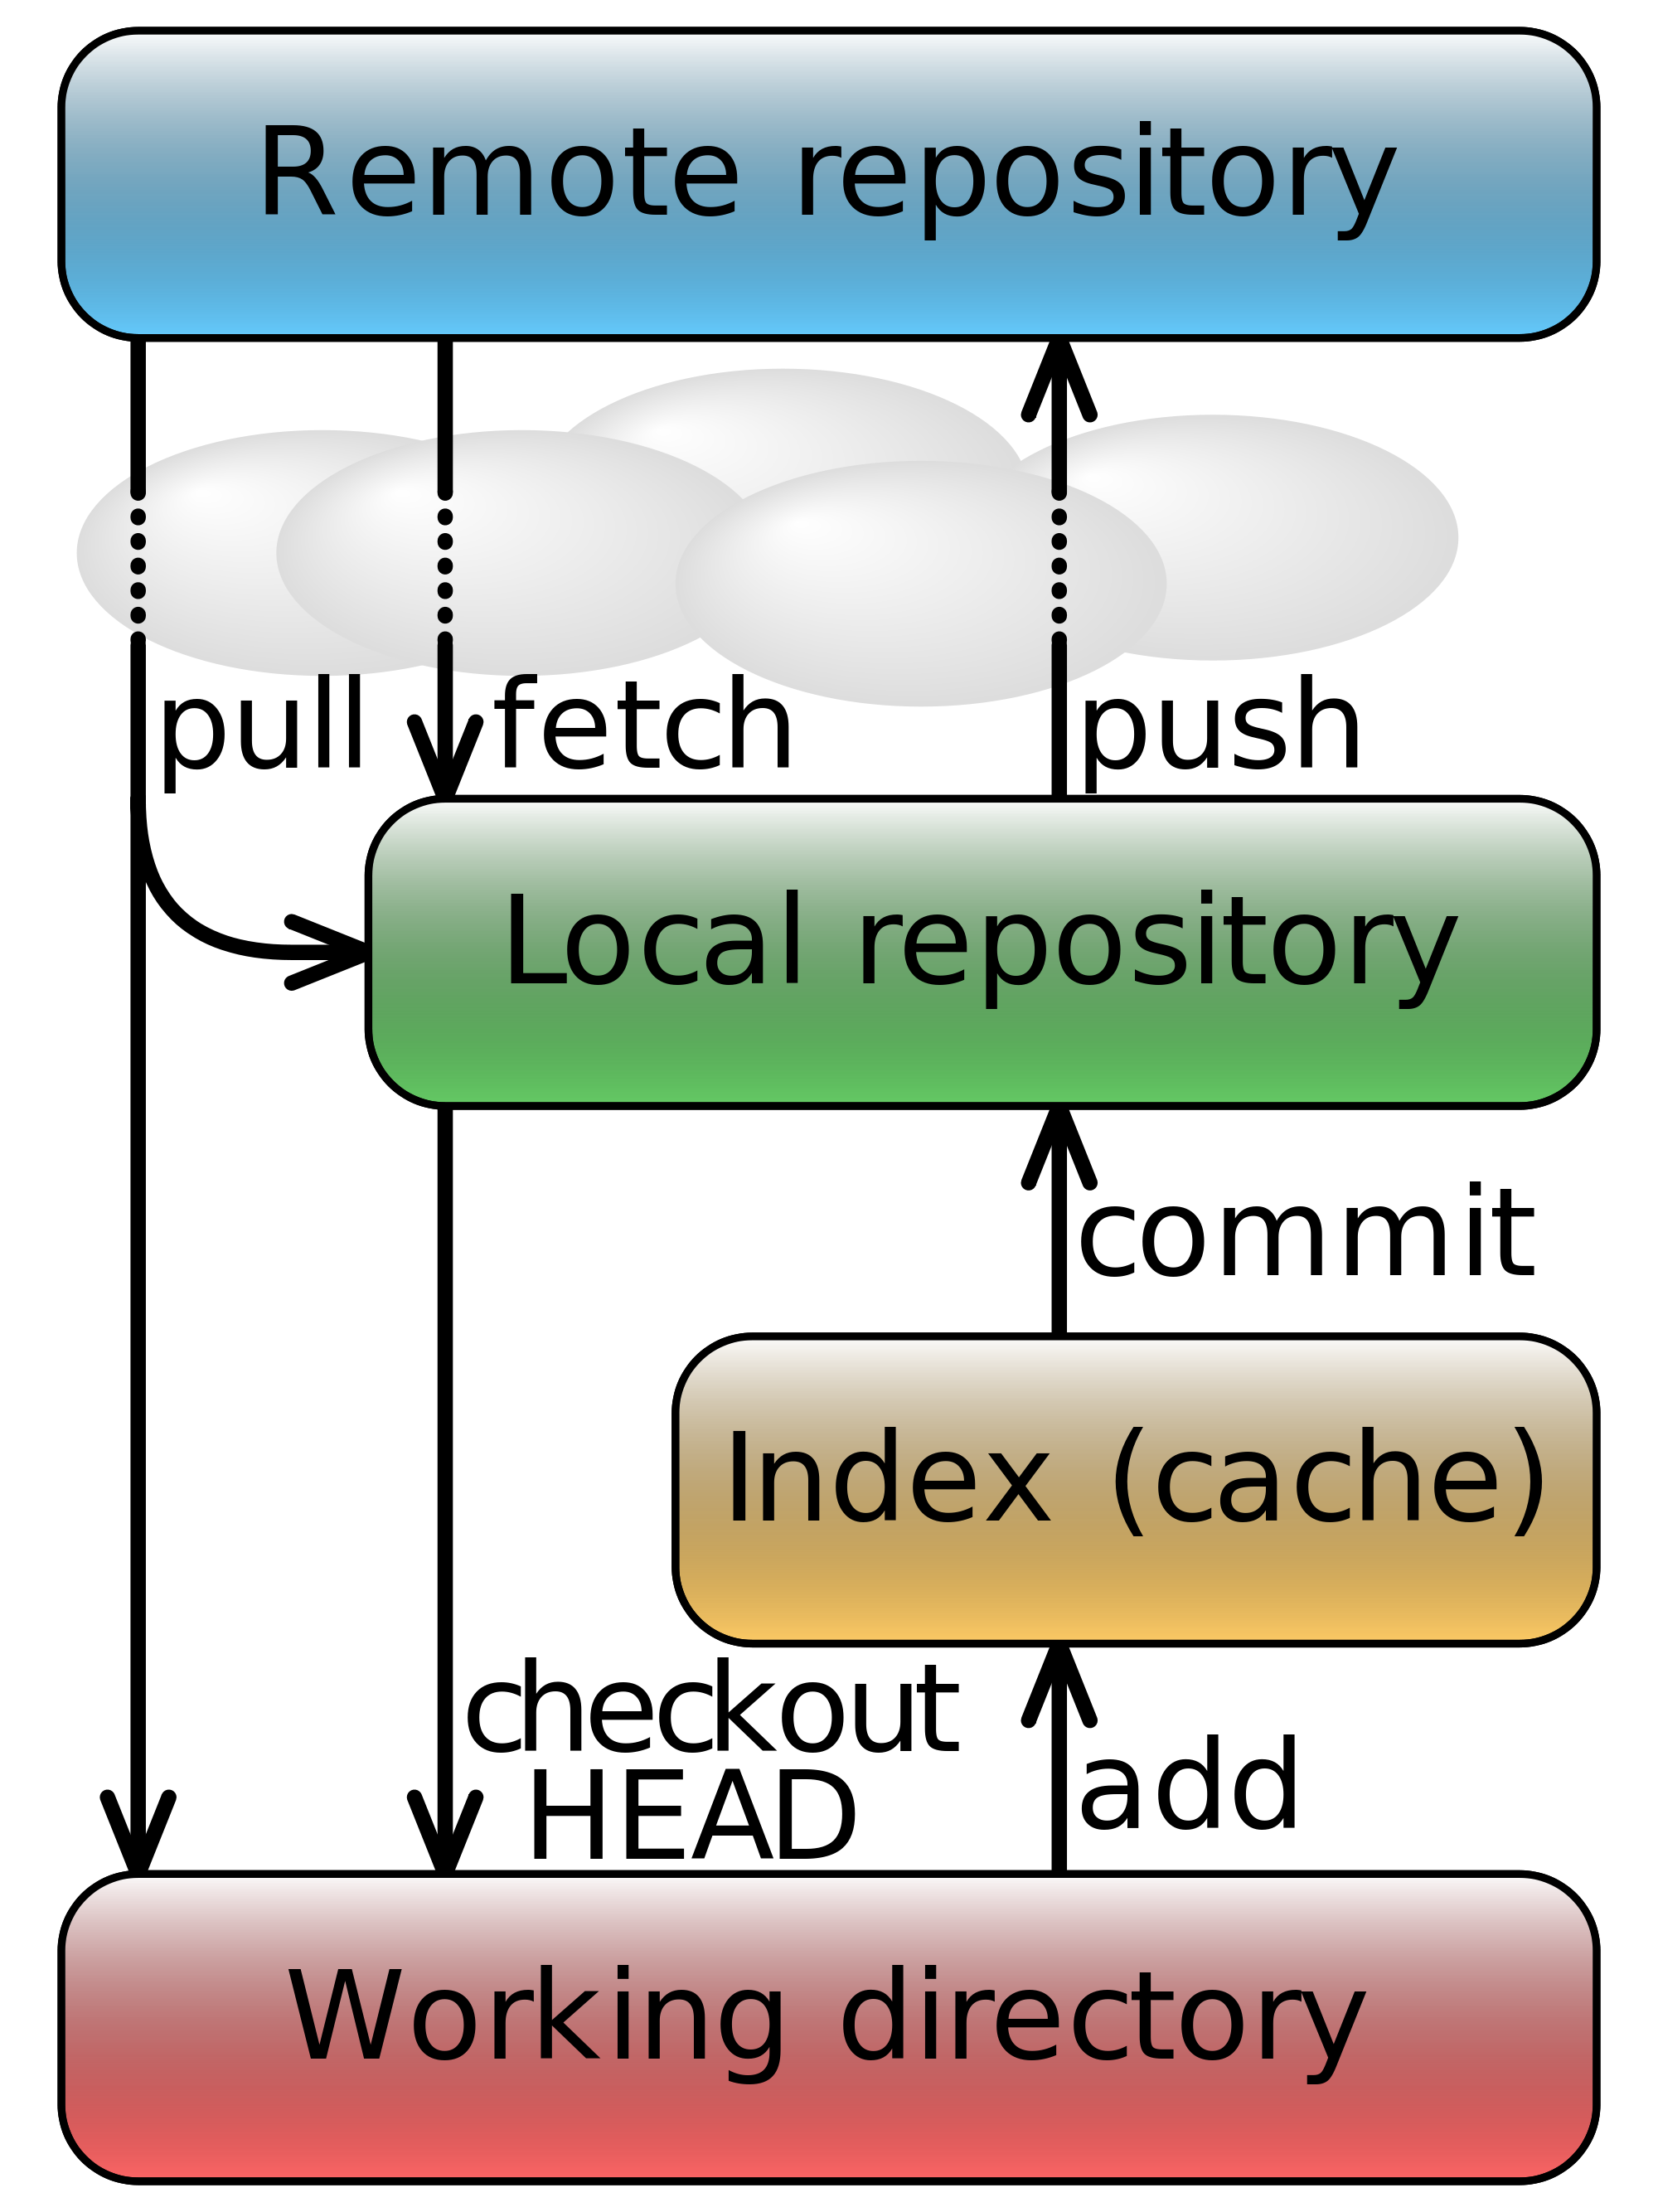
\includegraphics[height=8cm,keepaspectratio]{data/GitDataFlowSimplified.png}
            \label{pic:DataFlow}
        \column{4.5cm}
            \begin{itemize}
                \item 远程仓库
                \item 本地仓库
                \item 工作目录
            \end{itemize}
    \end{columns}
\end{frame}

\begin{frame}
    \frametitle{Git与CVS的部分区别
        \footnote{\scriptsize \url{http://stackoverflow.com/questions/802573/difference-between-git-and-cvs}}}
    \begin{block}{Git}
        \begin{itemize}
            \item 分布式仓库。用户无需任何服务器,在本地即可进行所有操作。
                  任何一个人的仓库,都可以做为远程仓库。
            \item 原子操作。操作要么完全成功,要么完全失败。
            \item 改动是对于整个项目。因此很容易回退到特定版本。
            \item 版本号也是基于整个项目。一个版本对应一个快照。
            \item 分支功能强大。包括创建合并等。
        \end{itemize}
    \end{block}
    \begin{block}{CVS}
        \begin{itemize}
            \item 集中式仓库。需要设置仓库的服务器,合并等操作都由服务器完成。
            \item 非原子操作。如果某个操作在中间被打断,可能处于不一致的状态。
            \item 改动是对于一个文件而言。我们可以checkout一些特定的文件。
            \item 版本号是对于特定文件。我们需要建立tag来指向特定的状态。
        \end{itemize}
    \end{block}
\end{frame}

\begin{frame}
    \frametitle{Git与SVN的部分区别
        \footnote{\scriptsize \url{http://stackoverflow.com/questions/871/why-is-git-better-than-subversion}}}
        \begin{quote}
            Git is not better than Subversion. But is also not worse. It's
            different.
        \end{quote}

        \begin{quote}
            The key difference is that it is decentralized.
        \end{quote}

        \begin{quote}
            Git has the advantage that it's MUCH better suited if some
            developers are not always connected to the master repository. Also,
            it's much faster than SVN. And from what I hear, branching and
            merging support is a lot better (which is to be expected, as these
            are the core reasons it was written).
        \end{quote}

        \begin{quote}
            SVN creates .svn directories in every single folder (Git only
            creates one .git directory). Every script you write, and every grep
            you do, will need to be written to ignore these .svn directories.
            You also need an entire command ("svn export") just to get a sane
            copy of your files.
        \end{quote}
\end{frame}

\begin{frame}
    \frametitle{Git使用时的建议\footnote{\scriptsize 仅为个人意见}}
    \begin{itemize}
        \item 为你的代码创建一个git仓库。可以只在本地。
              对可以公开的代码,可以托管于github等网站。
        \item 追踪你的代码。经常commit你的改动。
        \item 研究某一个新特性时,建立分支。最好在主干上创建分支。
        \item 多查资料。网上总有解答。
    \end{itemize}
    \begin{block}{我的一些经历体验}
        \begin{itemize}
            \item 在Dayabay SVN的people中提交过多commit,
                  导致邮件列表中出现太多的消息。我觉得这个hook不太好。
            \item 半年的Dyb2Sim开发,没有遇到太多git相关的问题。
                  唯一一次有难度的,是对geant4 9.4 和 9.5的同时支持。
                  因为geant4本身接口的变动,使得9.5环境下不可以直接编译9.4的代码。
                  开发某一个探测器时,是基于9.4,然后需要移到9.5。
                  感谢git,一条merge命令就搞定了。
        \end{itemize}
    \end{block}
\end{frame}
